\begin{figure}[H]
    \centering
    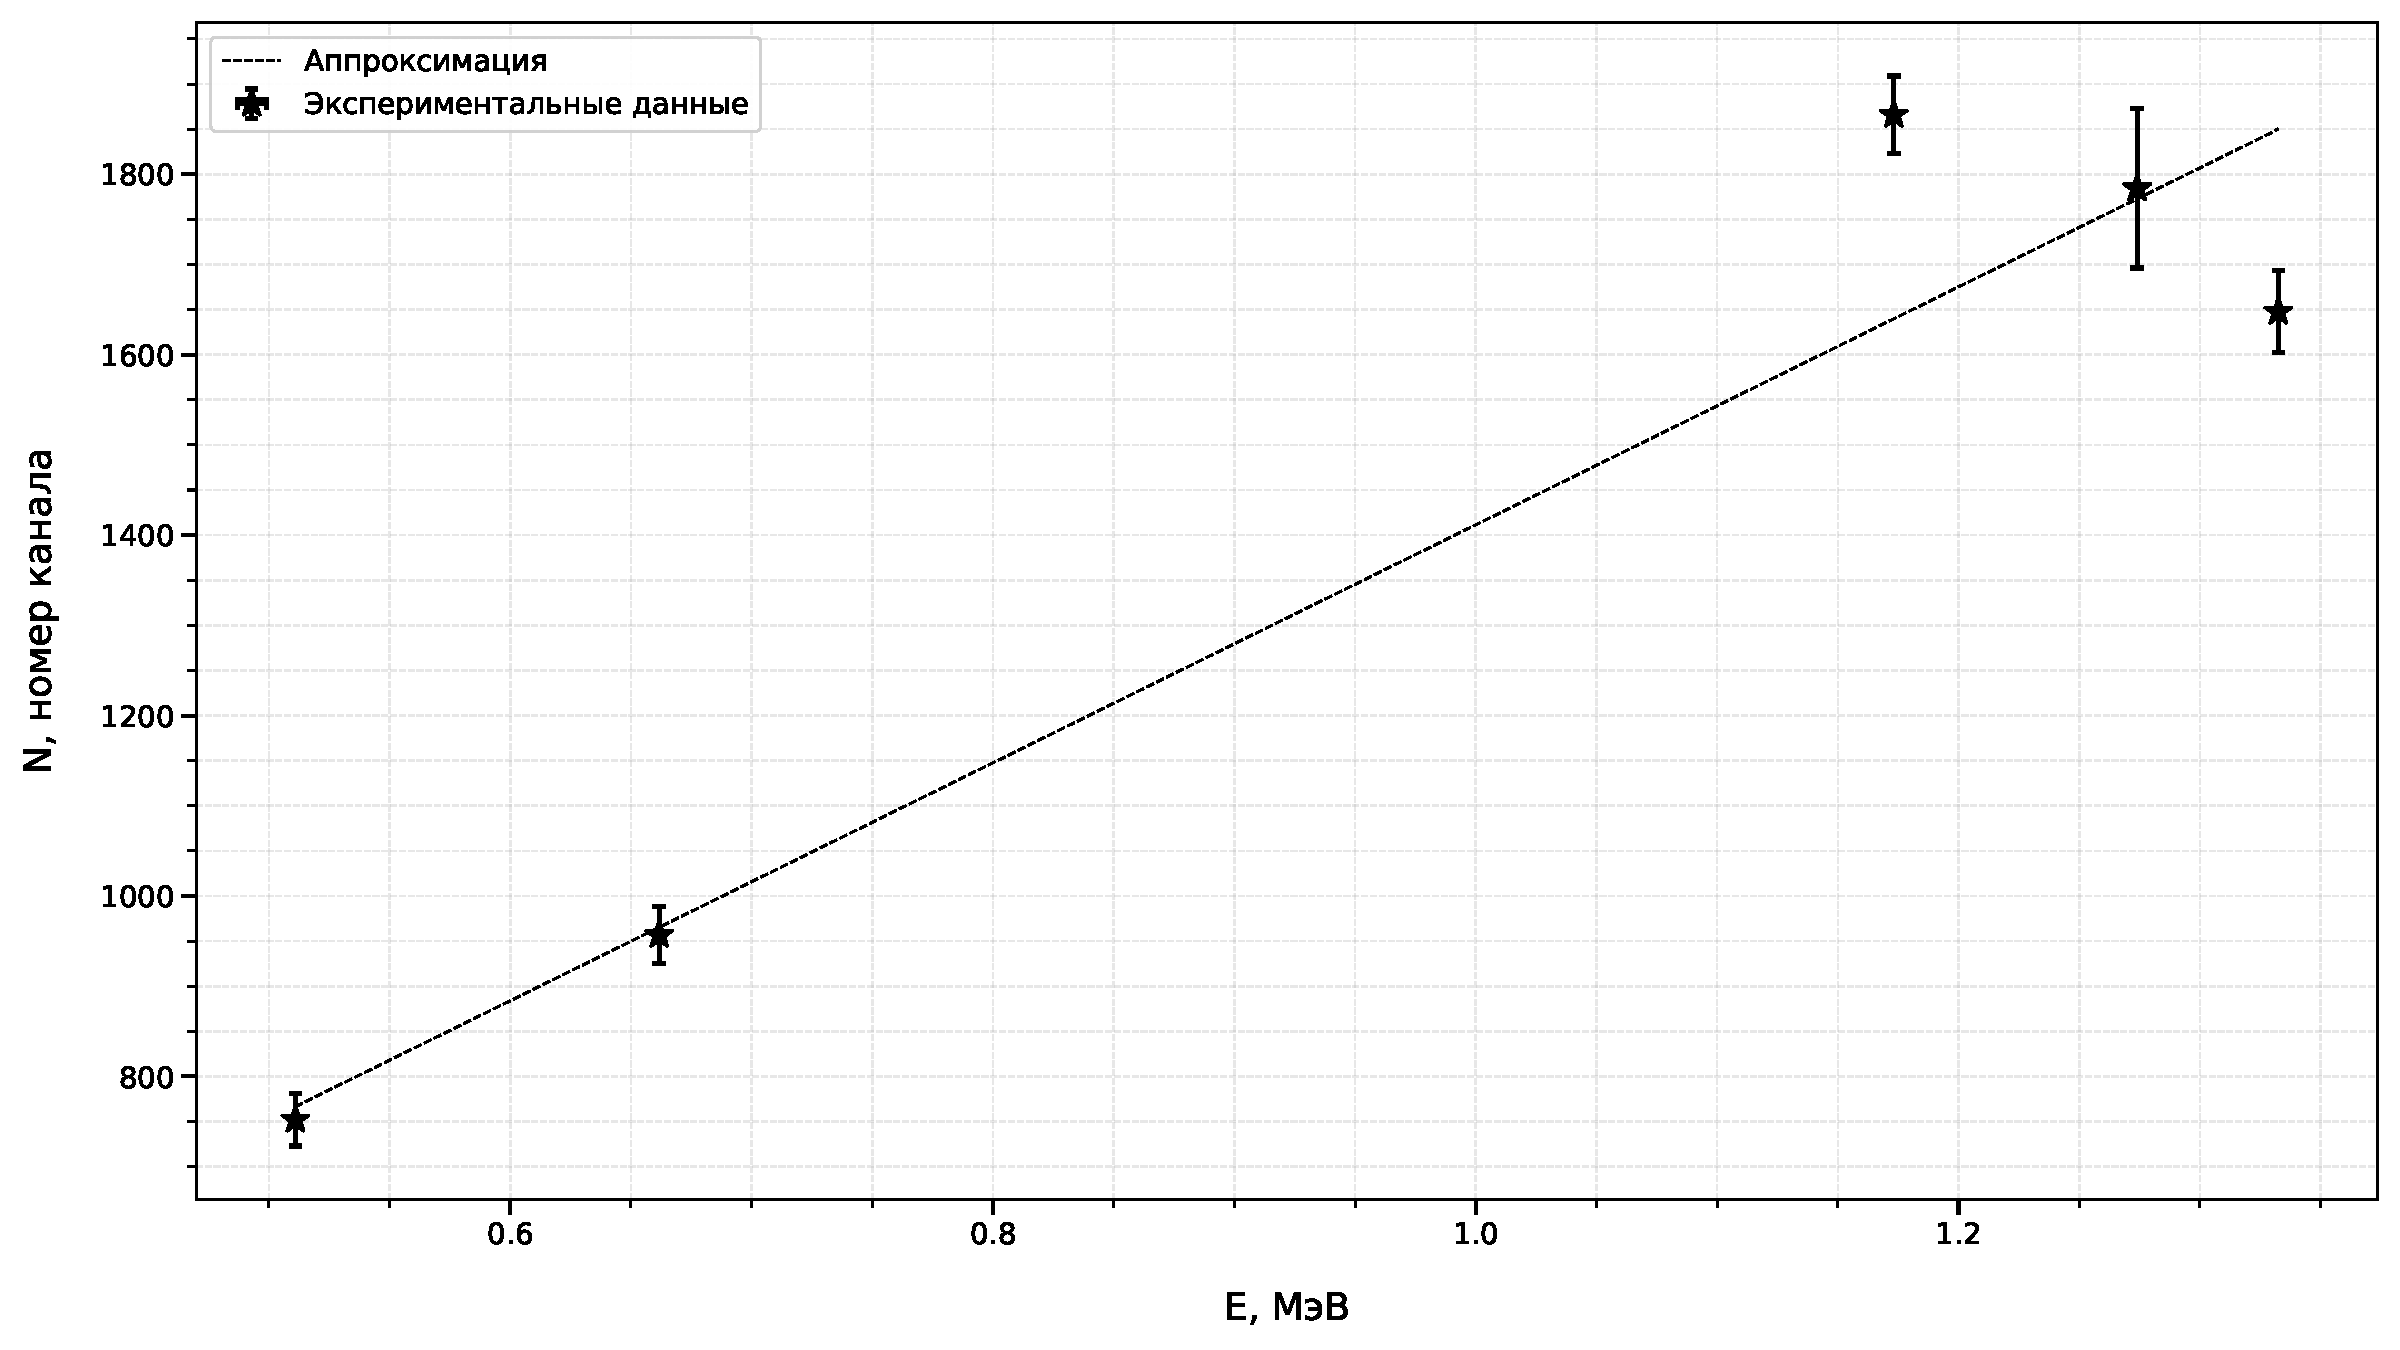
\includegraphics[width=1\textwidth]{pictures/calibrating} % Замените "example-image" на имя вашего файла изображения
    \caption{Калибровочный график $N_i = aE_i + b$}
    \label{}
\end{figure}

% Please add the following required packages to your document preamble:
% \usepackage{multirow}
% \usepackage[table,xcdraw]{xcolor}
% Beamer presentation requires \usepackage{colortbl} instead of \usepackage[table,xcdraw]{xcolor}
\begin{table}[]
\centering
\caption{Сводная таблица фотопиков}
\label{t1}
\begin{tabular}{|c|c|c|c|c|c|}
\hline
\rowcolor[HTML]{C6E0B4} 
Источник                     & $N_i$ & $\Delta N_i$ & $E_i, \text{   МэВ}$ & $\Delta E_i,   \text{ МэВ}$ & $R_i$ \\ \hline
                             & 1650  & 90           & 1.18                 & 0.07                        & 0.06  \\ \cline{2-6} 
\multirow{-2}{*}{$^{60}$Co}  & 1870  & 90           & 1.34                 & 0.07                        & 0.05  \\ \hline
$^{137}$Cs                   & 960   & 60           & 0.66                 & 0.05                        & 0.07  \\ \hline
                             & 750   & 60           & 0.50                 & 0.05                        & 0.08  \\ \cline{2-6} 
\multirow{-2}{*}{$^{22}$Na}  & 1790  & 90           & 1.28                 & 0.07                        & 0.05  \\ \hline
                             & 101   & 9            & 0.01                 & 0.04                        & 0.09  \\ \cline{2-6} 
\multirow{-2}{*}{$^{241}$Am} & 149   & 11           & 0.04                 & 0.04                        & 0.07  \\ \hline
                             & 117   & 16           & 0.02                 & 0.04                        & 0.14  \\ \cline{2-6} 
                             & 234   & 17           & 0.11                 & 0.04                        & 0.07  \\ \cline{2-6} 
\multirow{-3}{*}{$^{152}$Eu} & 530   & 40           & 0.33                 & 0.04                        & 0.08  \\ \hline
\end{tabular}
\end{table}

% Please add the following required packages to your document preamble:
% \usepackage{multirow}
% \usepackage{graphicx}
% \usepackage[table,xcdraw]{xcolor}
% Beamer presentation requires \usepackage{colortbl} instead of \usepackage[table,xcdraw]{xcolor}
\begin{sidewaystable}
\centering
\caption{Энергия края комптоновского рассеяния для разных источников}
\label{t2}
% Убран resizebox, так как таблица, скорее всего, поместится в повернутом виде
\begin{tabular}{|c|c|c|c|c|c|}
\hline
\rowcolor[HTML]{C6E0B4} 
{\color[HTML]{1B1C1D} Источник} & $E_{\text{пк}} (\text{МэВ})$ & $\sigma_{E_{\text{пк}}} (\text{МэВ})$ & $E^{\text{theor}}_{\text{пк}} (\text{МэВ})$ & $\sigma^{\text{theor}}_{E_{\text{пк}}} (\text{МэВ})$ & Комментарий \\ 
\hline
$^{60}$Co & 0.92 & 0.07 & 0.97 & 0.07 & От левого фотопика \\ 
\hline
$^{137}$Cs & 0.44 & 0.05 & 0.47 & 0.05 & От фотопика \\ 
\hline
\multirow{-2}{*}{$^{22}$Na} & 0.29 & 0.05 & 0.33 & 0.04 & От аннигиляционного фотопика \\ 
\cline{2-6} 
 & 1.11 & 0.07 & 1.07 & 0.07 & От фотопика \\ 
\hline
\end{tabular}
\end{sidewaystable}

\begin{figure}[H]
    \centering
    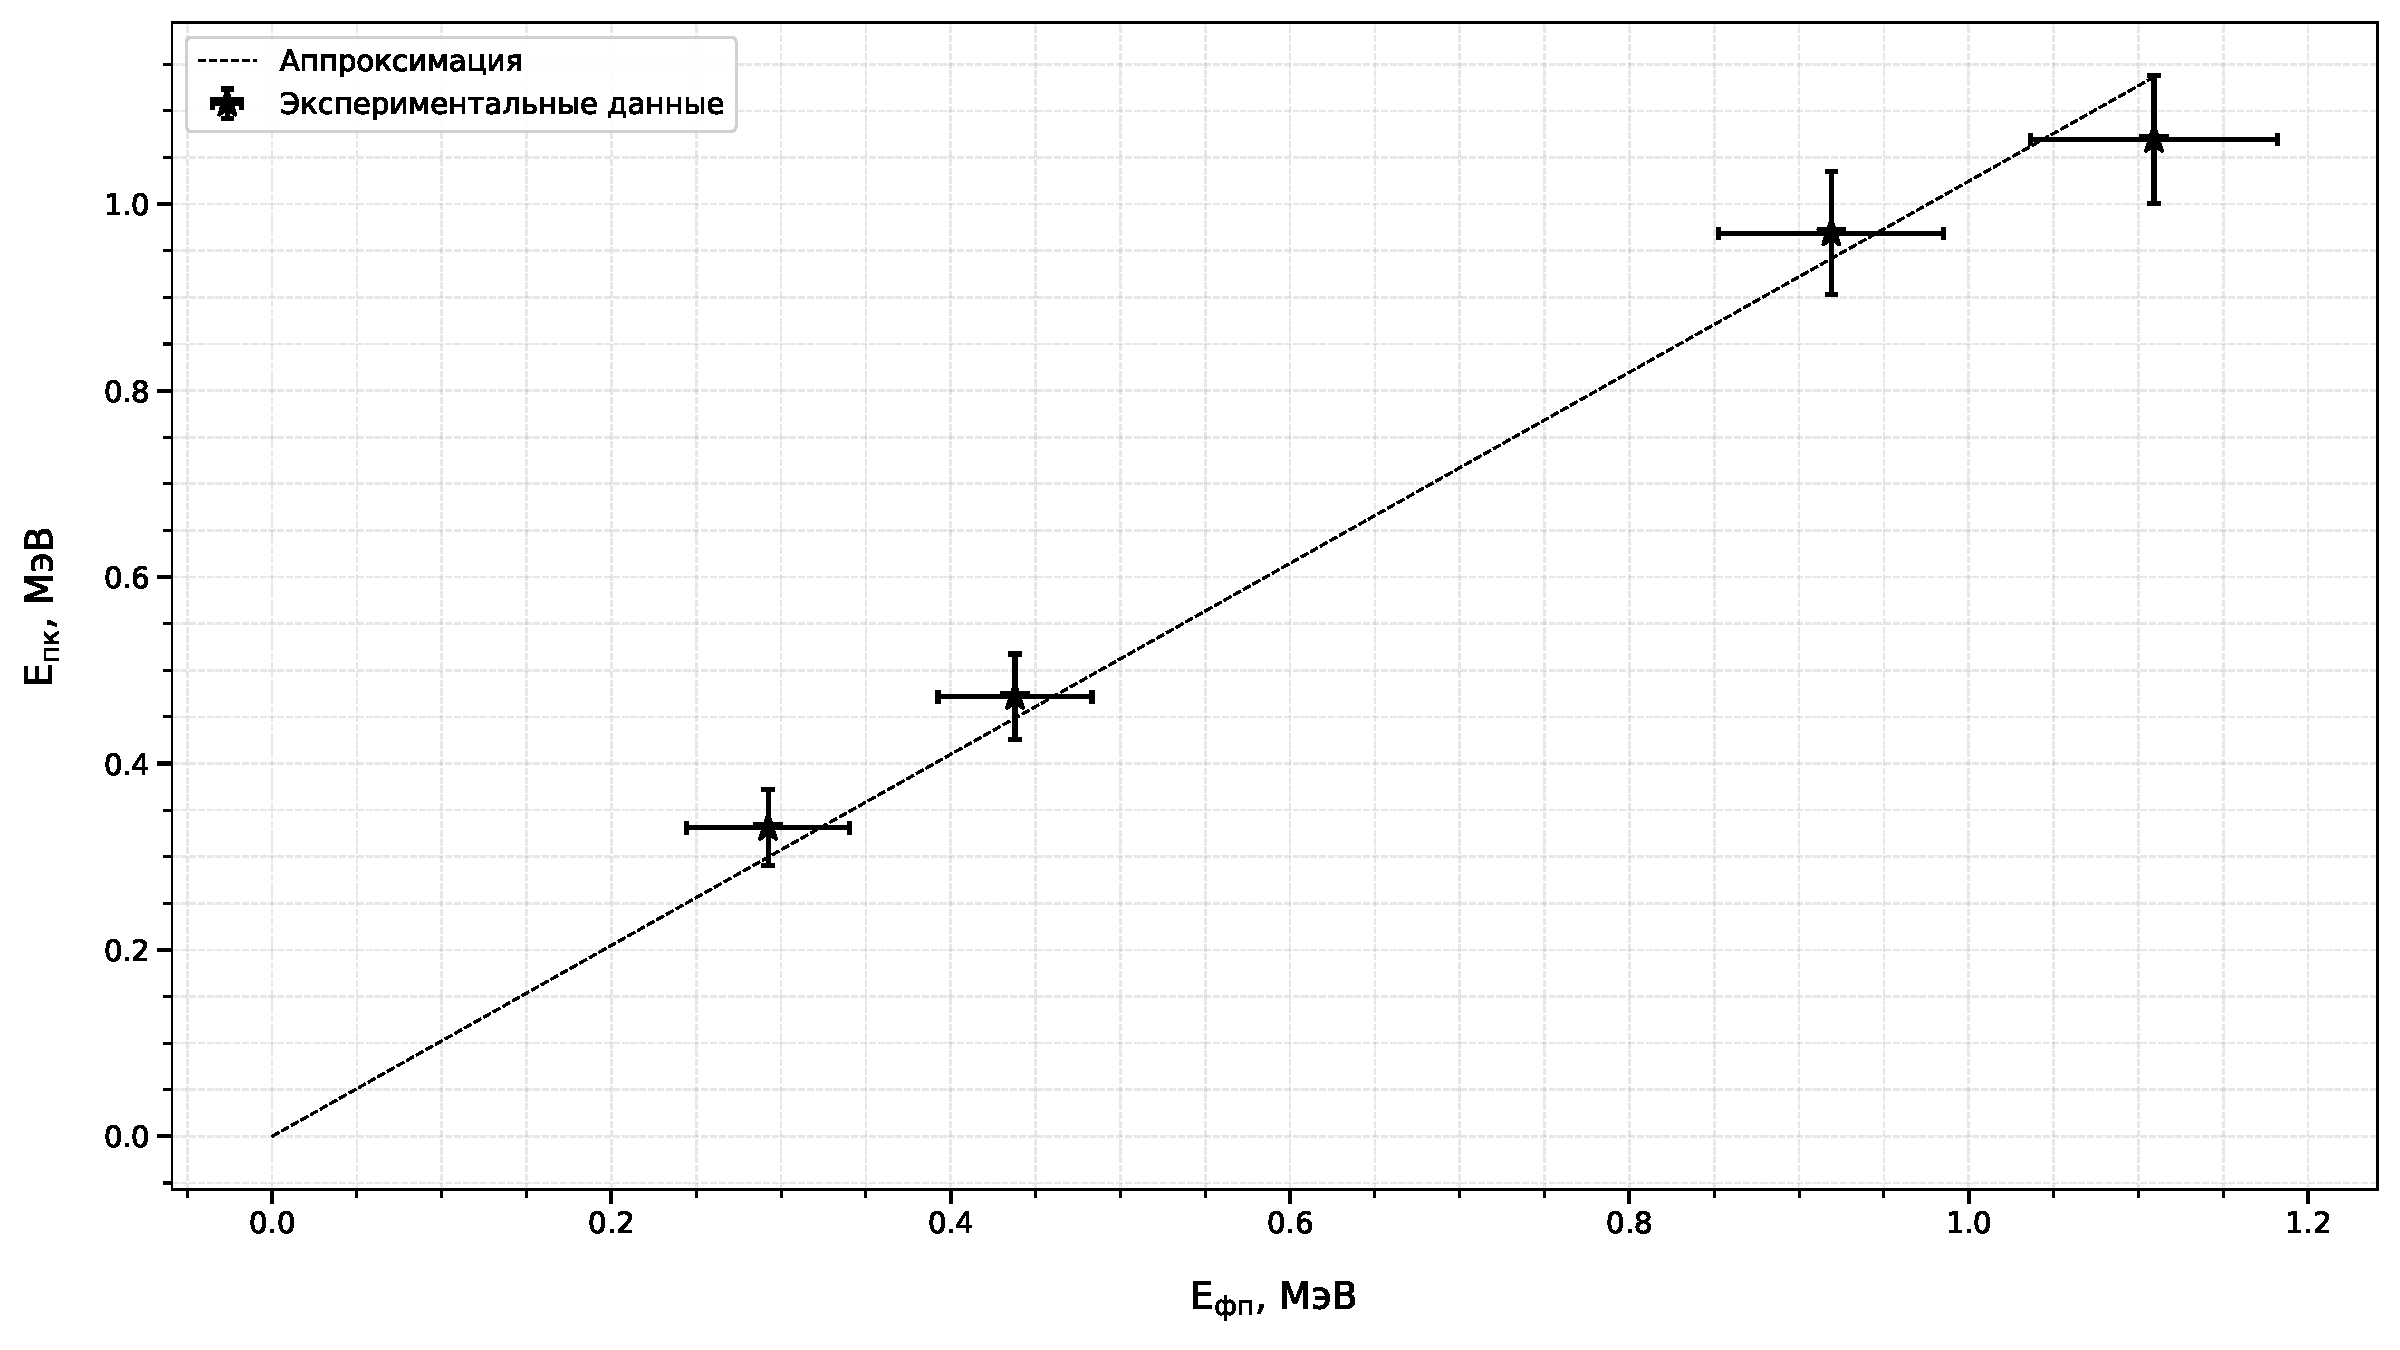
\includegraphics[width=1\textwidth]{pictures/compton_comparation} % Замените "example-image" на имя вашего файла изображения
    \caption{Сравнение экспериментальных и теоретических значений максимальной энергии комптоновского рассеяния}
    \label{}
\end{figure}

\begin{figure}[H]
    \centering
    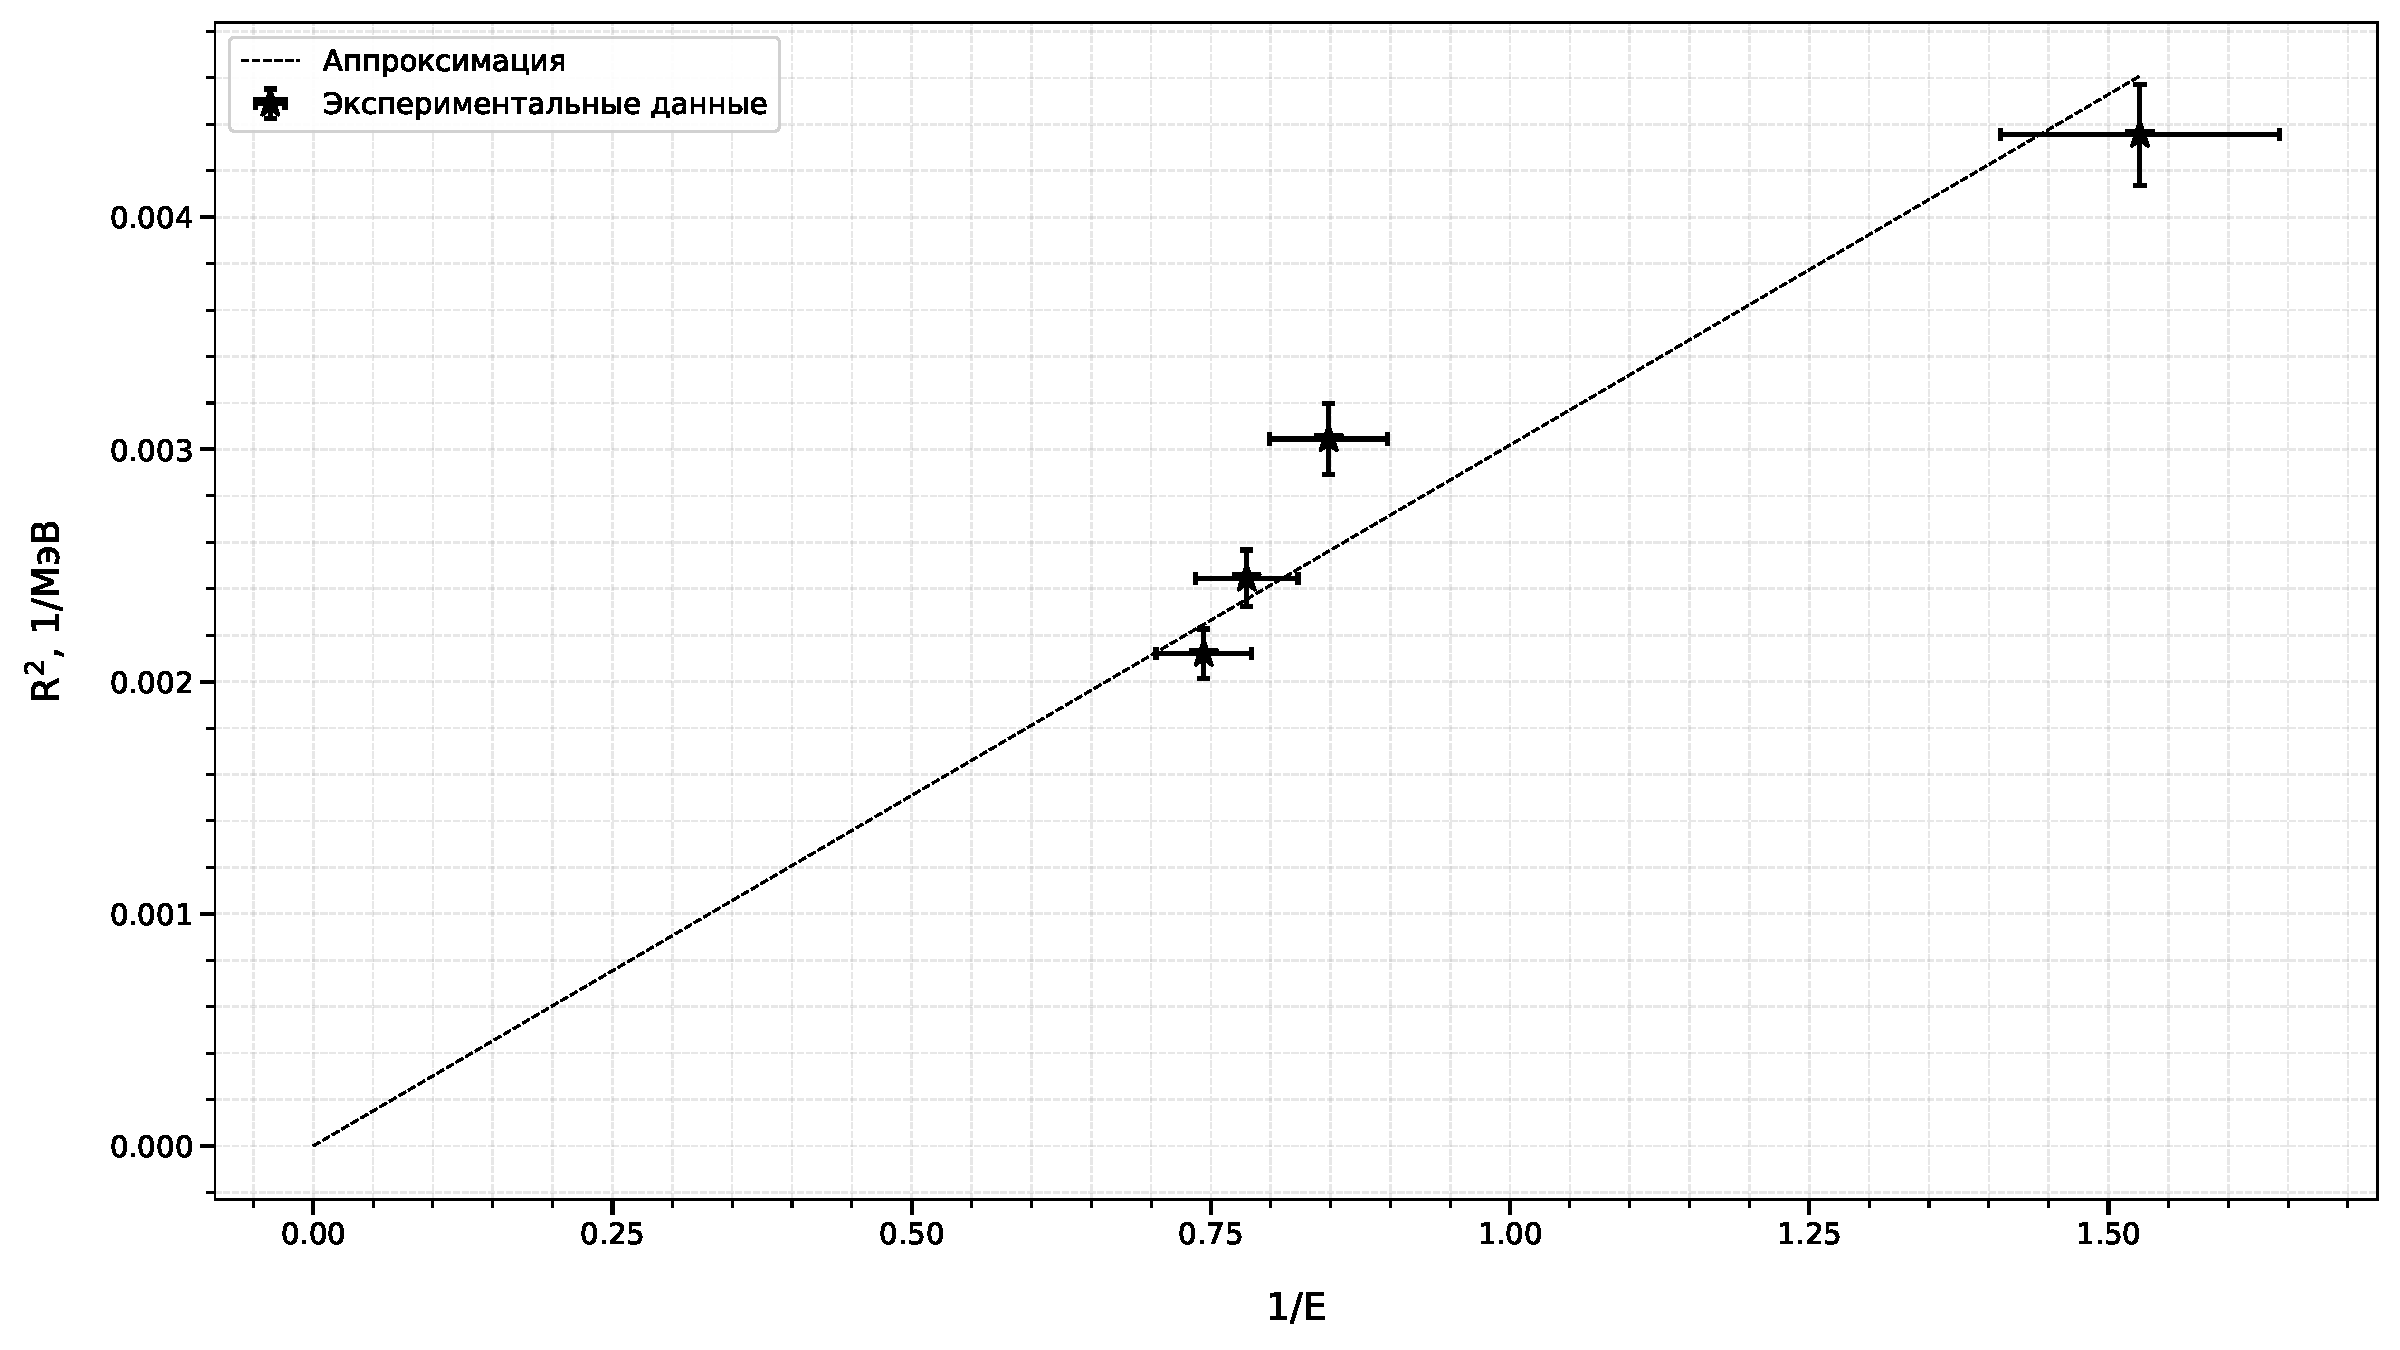
\includegraphics[width=1\textwidth]{pictures/spectrometer_resolution} % Замените "example-image" на имя вашего файла изображения
    \caption{Сравнение экспериментальных и теоретических значений энергетического разрешения спектрометра}
    \label{}
\end{figure}

\begin{figure}[H]
    \centering
    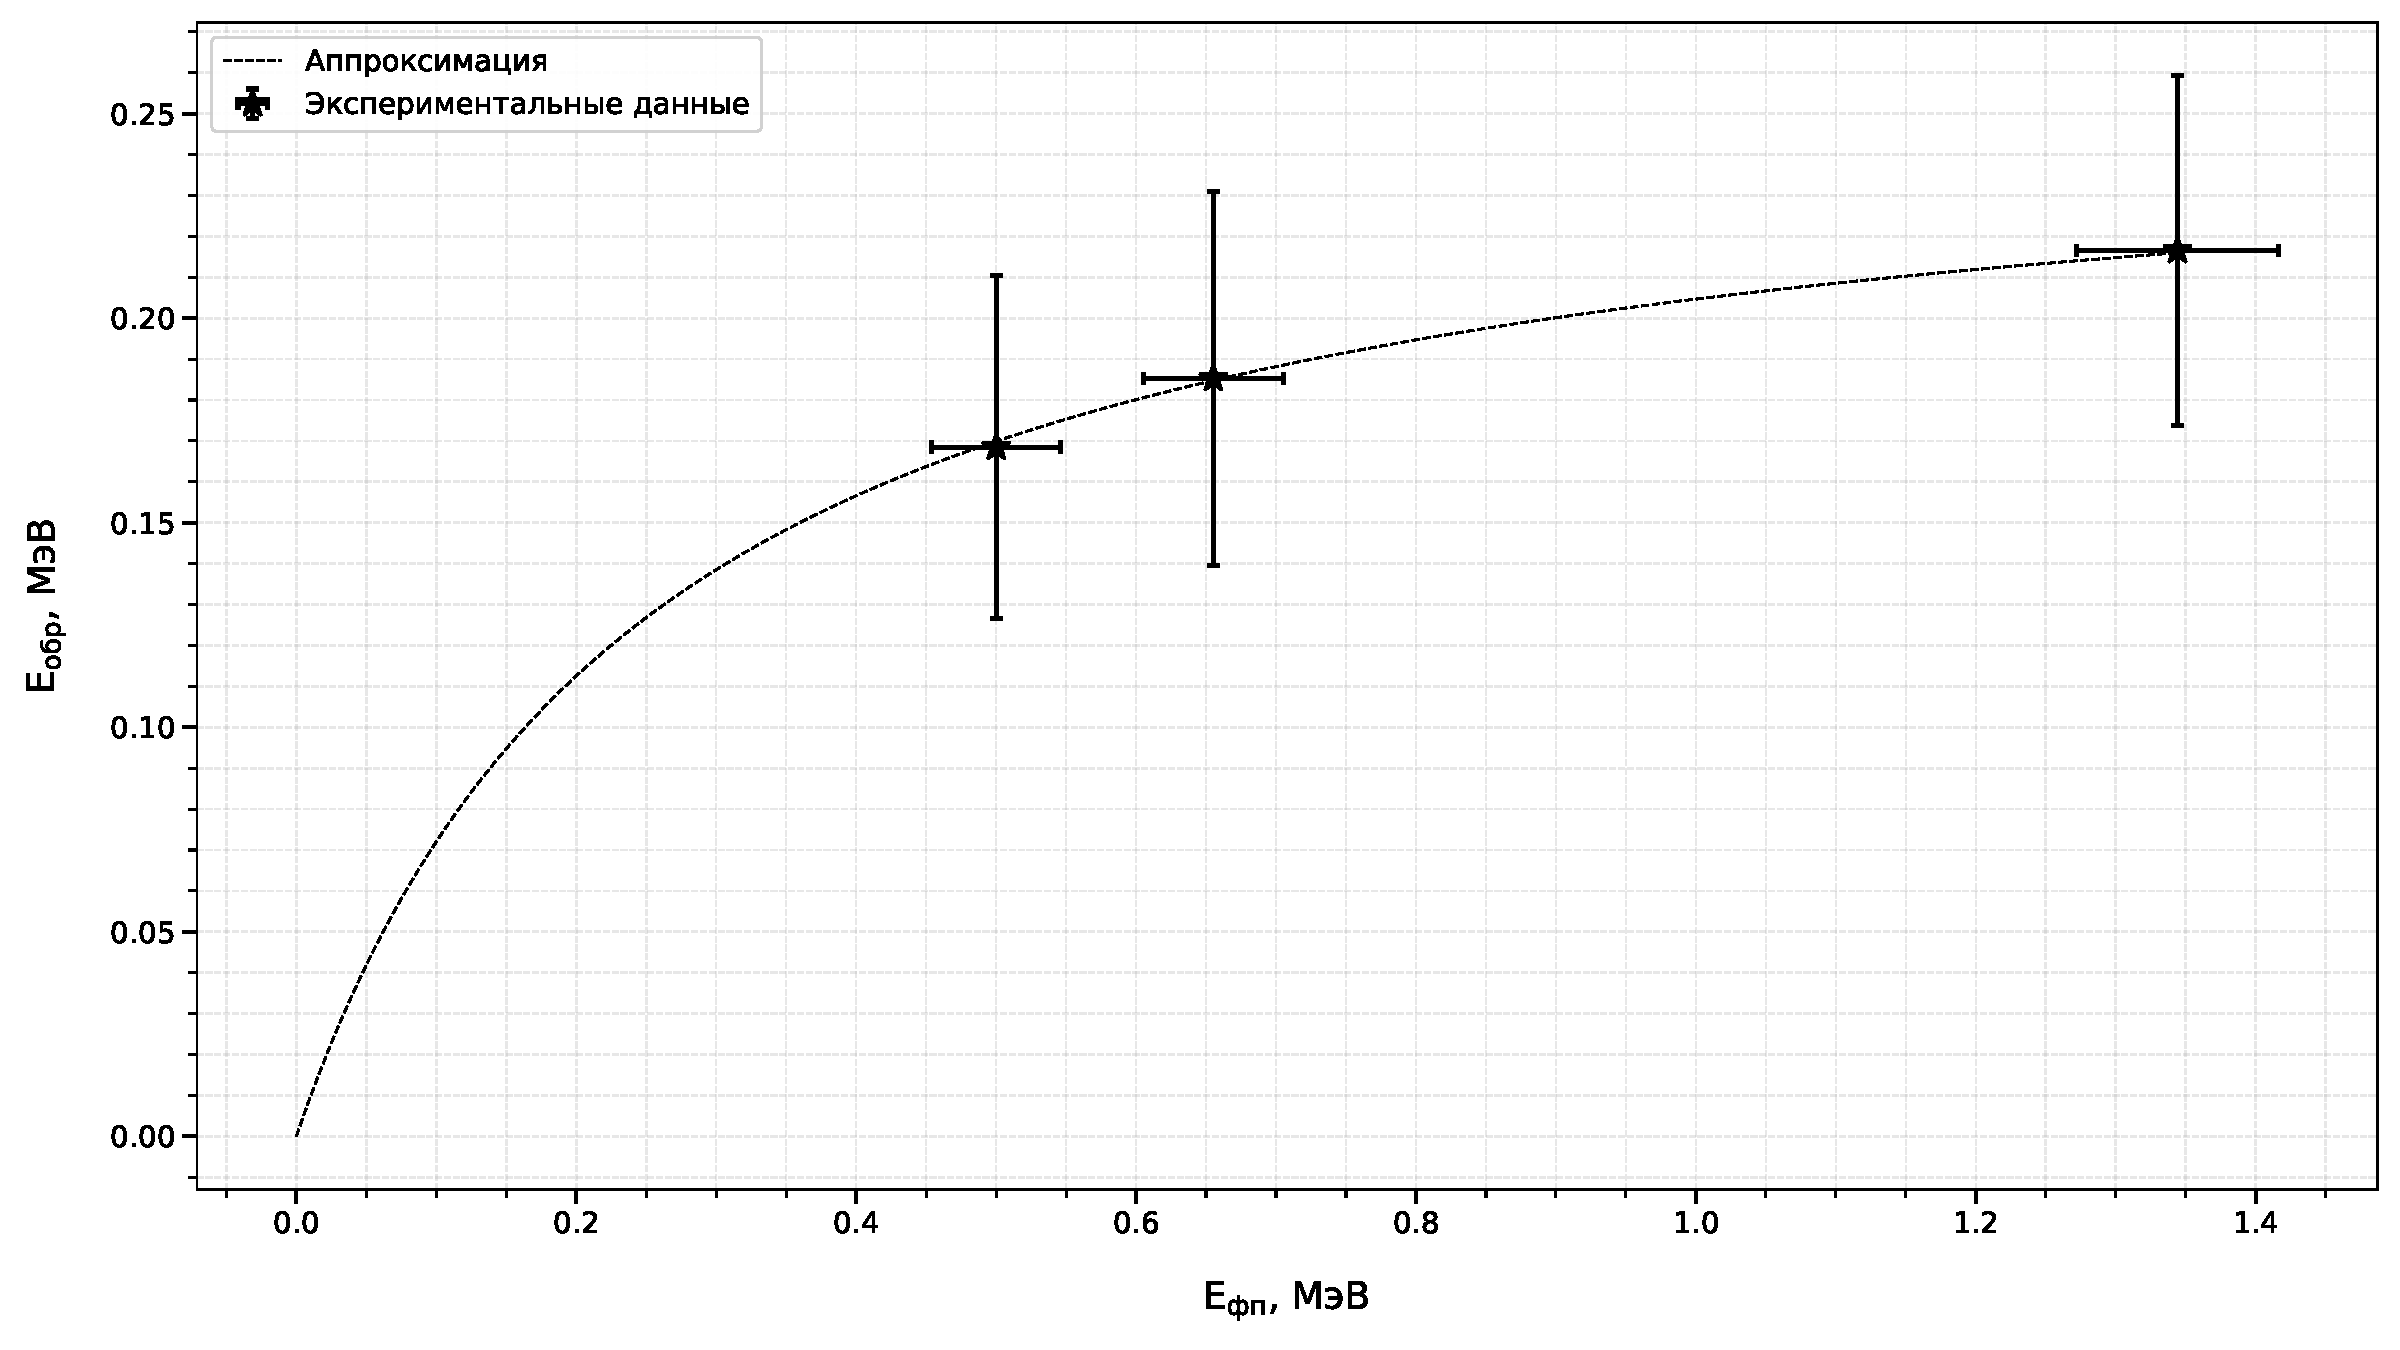
\includegraphics[width=1\textwidth]{pictures/backward_scattering} % Замените "example-image" на имя вашего файла изображения
    \caption{Зависимость пика обратного комптоновского рассеяния от энергии фотопика}
    \label{}
\end{figure}